\section{Interferometric stabilisation of reservoir cavity}

\begin{frame}{Interferometry}
	
\end{frame}

\begin{frame}{Experimental setup}
	\begin{figure}
		\centering
		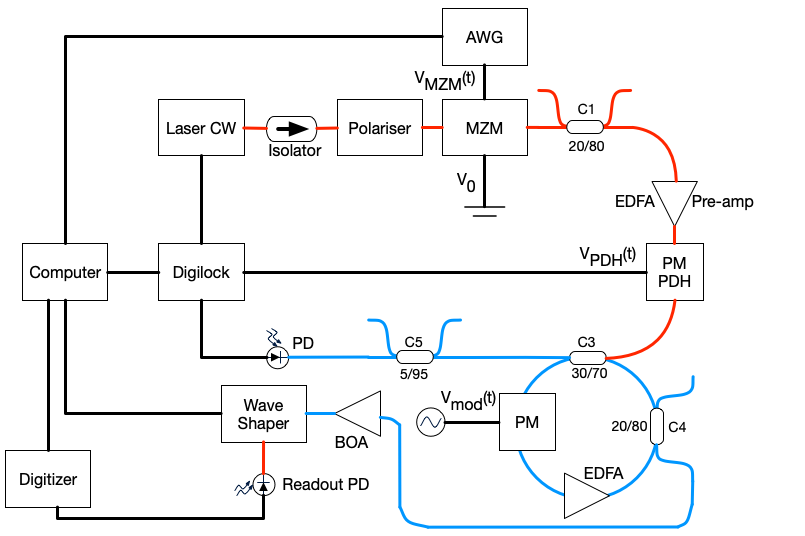
\includegraphics[width=.85\textwidth]{exp-setup.png}
	\end{figure}
\end{frame}

\begin{frame}{Transfer function of the cavity}
	\begin{figure}
		\centering
		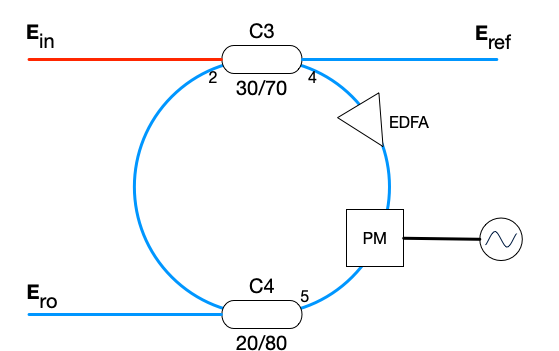
\includegraphics[width=.6\textwidth]{reservoir.png}
		\begin{itemize}
			\item \textbf{Transfer matrix} of the cavity :
			\begin{equation*}
				\mathbf{E}_{\text{ref}} = \mathbf{R} ~\mathbf{E}_{\text{in}}
			\end{equation*}
		\end{itemize}
		\begin{alertblock}{}
			\begin{equation*}
				\mathbf{R} = \epsilon_1 \mathbf{I} - (1-\epsilon_1^2) \epsilon_2 e^{-\gamma L} \left( \mathbf{I} - \epsilon_1 \epsilon_2 e^{- \gamma L} \Phi_{1-\xi} \mathbf{J} \Phi_\xi \right)^{-1} \Phi_{1-\xi} \mathbf{J} \Phi_\xi
			\end{equation*}
		\end{alertblock}

	\end{figure}
\end{frame}

\begin{frame}{Transfer function of the cavity}
	\begin{itemize}
		\item Reflected field for a monochromatic input field:
		\begin{equation*}
			\mathbf{E}_{\text{ref}} = E_0 \sum_{n=-\eta}^\eta R_{n,0} \hat{\mathbf{e}}_n \Longrightarrow |\mathbf{E}_{\text{ref}}|^2 \approx |E_0|^2 \sum_{n=-\eta}^\eta |R_{n,0} |^2
		\end{equation*}
		\item Reflectivity :
		\begin{equation*}
			\mathcal{R}(\omega) = \sum_{n=-\eta}^\eta |R_{n,0} (\omega) |^2
		\end{equation*}
	\end{itemize}
	\begin{columns}
		\begin{column}{.5\textwidth}
			\begin{figure}
				\centering
				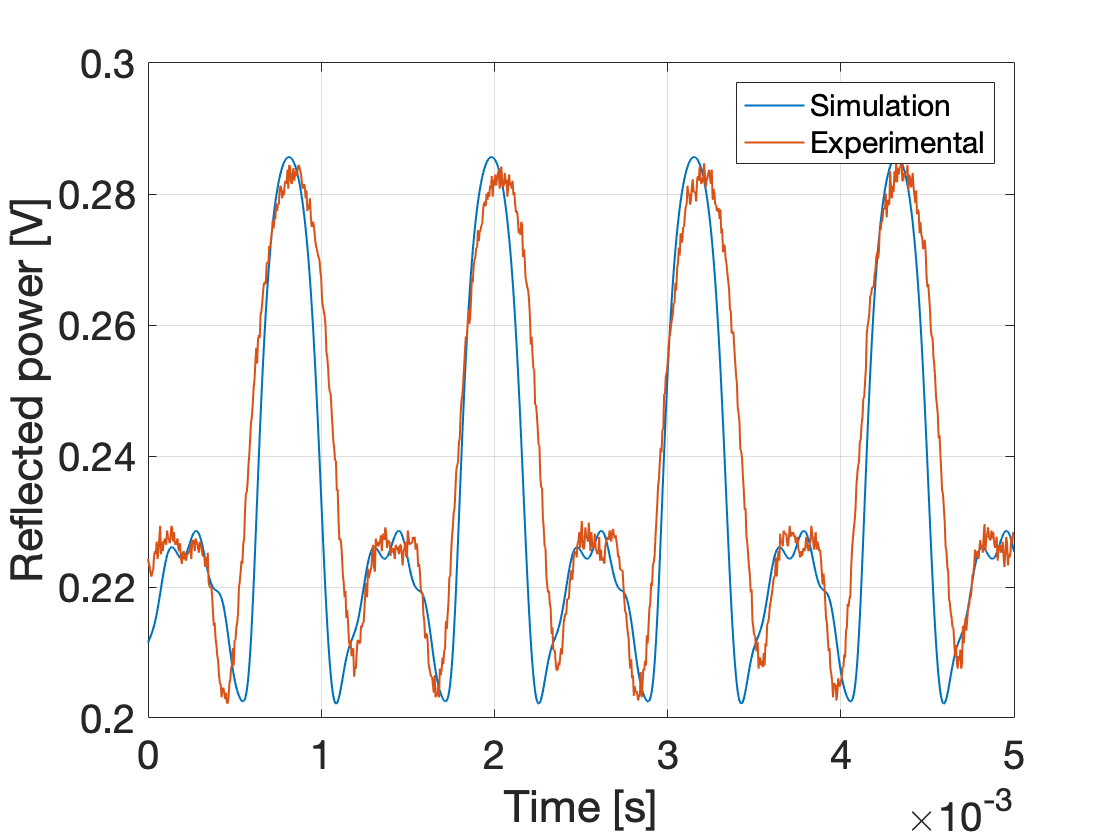
\includegraphics[width=.8\textwidth]{tf_0.png}
			\end{figure}	
		\end{column}%
		\begin{column}{.5\textwidth}
			\begin{figure}
				\centering
				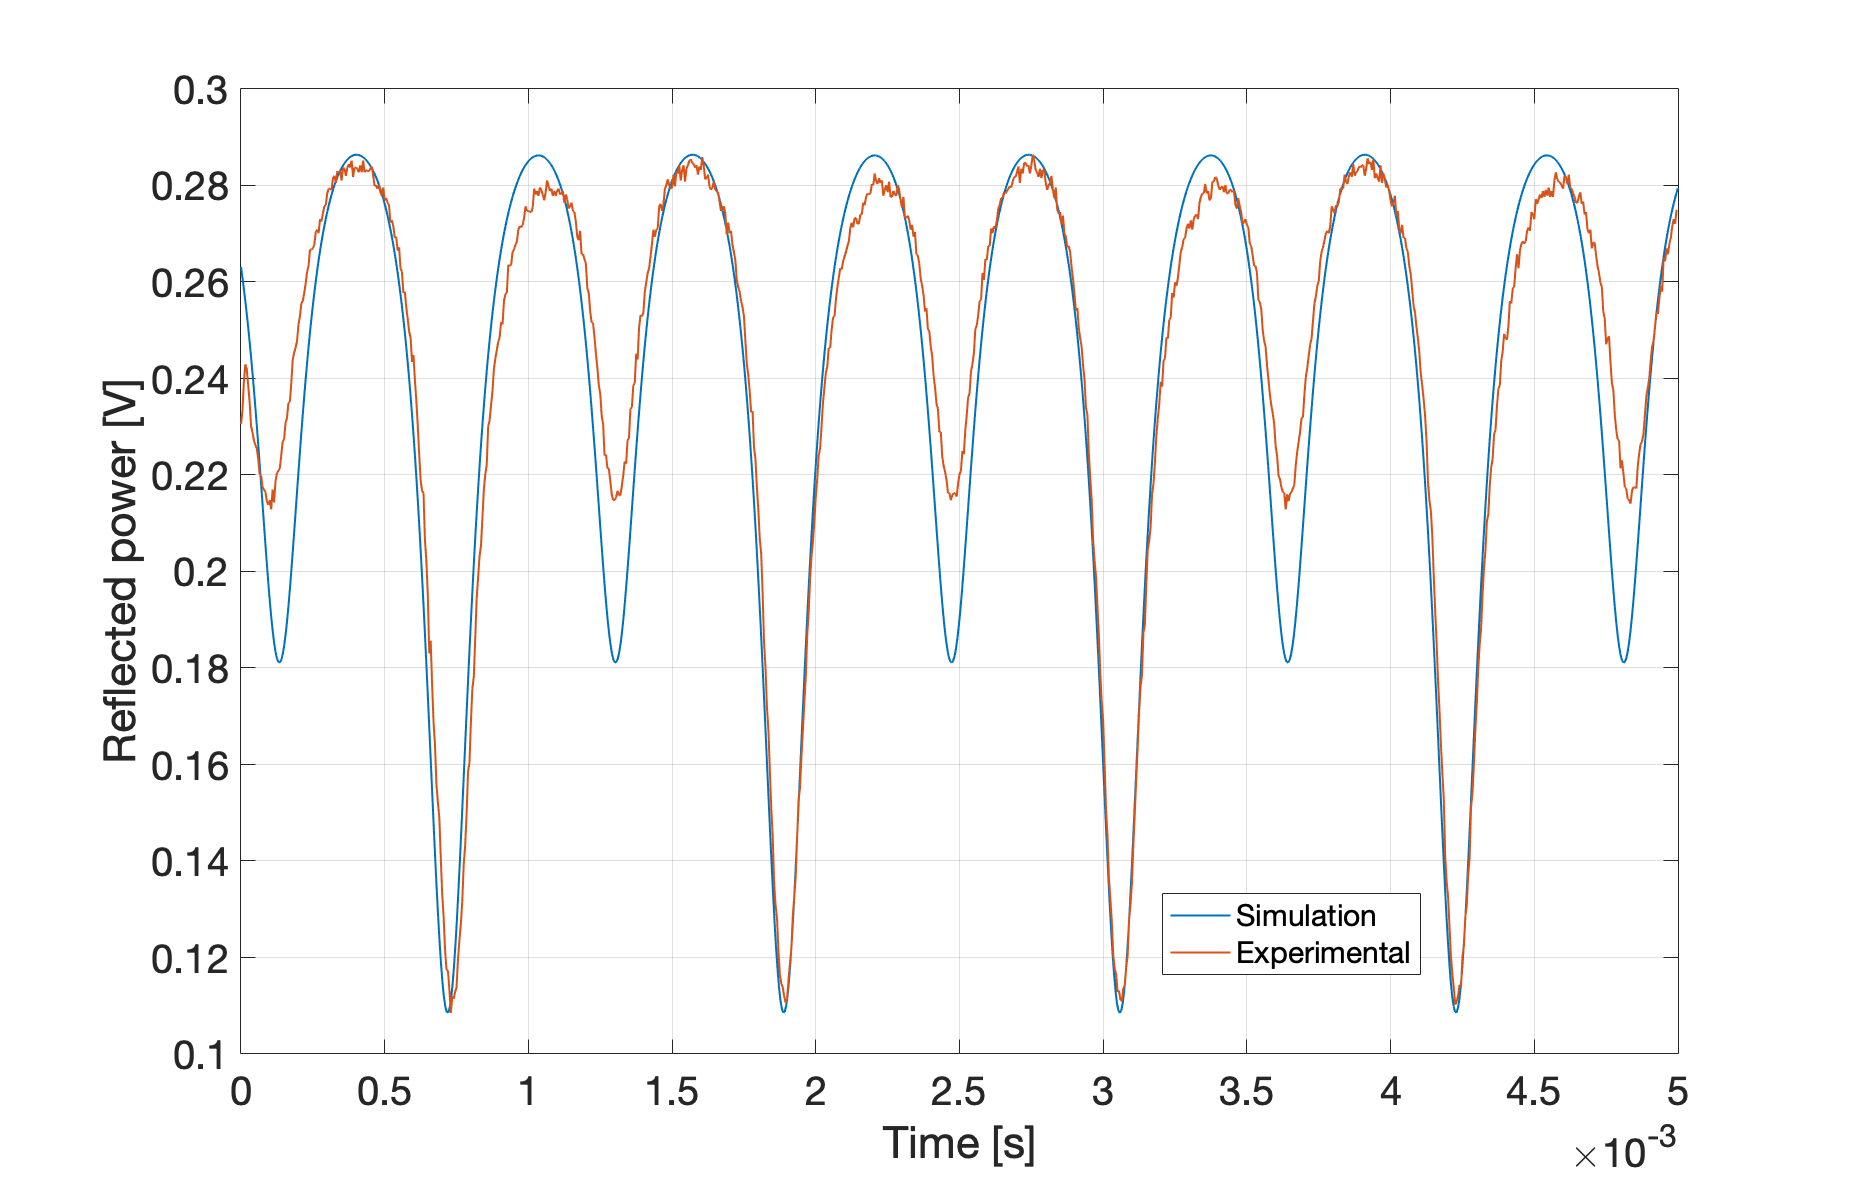
\includegraphics[width=.8\textwidth]{tf_50.png}
			\end{figure}	
		\end{column}
	\end{columns}
\end{frame}

\begin{frame}{Classical cavity stabilisation}
	
\end{frame}

\begin{frame}{Pound-Drever-Hall technique}
	
\end{frame}

\begin{frame}{Pound-Drever-Hall technique for the reservoir cavity}

\end{frame}

\begin{frame}{Cavity stabilisation performances}
	
\end{frame}

\begin{frame}{Results}

	\begin{table}
		\centering
			\begin{tabular}{|c|c|c|c|c|c|}
				\hline
				\small{Rank} & $A_{\text{PDH}}$ [\si{\voltptp}] & $\nu_{\text{PDH}}$ [\si{\kilo\hertz}] & $\epsilon^*$ [\si{\au}] & $\phi$ [\si{\radian}] & \small{Challenger} [\si{\milli\radian\squared}]\\
				\hline
				\hline
				\#1 & 0.4 & 781 & 400 & 1.3 & 291.5\\
				\#2 & 0.2 & 781 & -300 & -1.43 & 327\\
				\#3 & 0.4 & 781 & 700 & 1.45 & 337.25\\
				\#4 & 0.3 & 781 & 500 & 1.31 & 362.25\\
				\#5 & 0.4 & 781 & 600 & 1.39 & 376.5\\
				\hline
			\end{tabular}
	\end{table}
	
	\begin{itemize}
		\item Overall best modulation frequency $\nu_{\text{PDH}} = \SI{781}{\kilo\hertz}$
		\item However, measurements of modulation amplitudes are inconsistant
		\begin{itemize}
			\item Should not depend on the stabilisation position
			\item Most probable explanation : software developed to post-process raw data not working properly
		\end{itemize}
	\end{itemize}
	
\end{frame}